\documentclass[a4paper,fleqn]{cas-dc}

\usepackage[utf8]{inputenc}
\usepackage[T1]{fontenc}
\usepackage[expansion=false]{microtype}
\usepackage{amsmath,amssymb}
\usepackage{booktabs}
\usepackage{graphicx}
\usepackage{multirow}
\usepackage{tabularx}
\usepackage{placeins}
\usepackage{xspace}
\usepackage{tikz}
\usetikzlibrary{arrows.meta,positioning,shapes.geometric,fit}
\usepackage[ruled,vlined,linesnumbered]{algorithm2e}
\usepackage[numbers,sort&compress]{natbib}
\usepackage{xcolor}
\usepackage{hyperref}

\hypersetup{
  colorlinks=true,
  linkcolor=blue,
  citecolor=blue,
  urlcolor=blue
}

\newcommand{\method}{NARCIS\xspace}
\newcommand{\bits}{\mathrm{bpc}}
\newcolumntype{Y}{>{\raggedright\arraybackslash}X}

\begin{document}
\let\WriteBookmarks\relax
\def\floatpagepagefraction{1}
\def\textpagefraction{.001}

\shorttitle{Authenticated Neural Coverless Image Signaling}
\shortauthors{Ekodeck \textit{et al.}}

\title[mode=title]{NARCIS: Authenticated Neural Coverless Image Signaling with Attack-Qualified Codebooks and Error Correction}

\author[1,2,3]{St\'ephane Ga\"el R. Ekodeck}[
  orcid=0000-0002-8094-8832]
\cormark[1]
\ead{stephane-gael.ekodeck@facsciences-uy1.cm}
\credit{Conceptualization, Methodology, Software, Validation, Formal analysis,
Investigation, Data curation, Visualization, Writing -- original draft}

\author[4,5]{Vivien Beyala Kamgang}[
  orcid=0000-0002-3644-1866]
\ead{vivsxx@univ-bertoua.cm}
\credit{Conceptualization, Methodology, Writing -- review and editing}

\author[1,2,3]{Serge Alain Eb\'el\'e}[
  orcid=0000-0001-7036-7068]
\ead{serge-alain.ebele@facsciences-uy1.cm}
\credit{Conceptualization, Methodology, Validation, Writing -- review and
editing}

\author[5,4]{Julius Marcellin Nkenlifack}[
  orcid=0000-0003-3322-4687]
\ead{marcellin.nkenlifack@gmail.com}
\credit{Supervision, Project administration, Writing -- review and editing}

\affiliation[1]{
  organization={Department of Computer Science, LIRIMA, TEAM GRIMCAPE,
  University of Yaound\'e I},
  addressline={P.O. Box 812},
  city={Yaound\'e},
  country={Cameroon}
}
\affiliation[2]{
  organization={IRD, UMI 209 UMMISCO, IRD France Nord},
  city={Bondy},
  postcode={F-93143},
  country={France}
}
\affiliation[3]{
  organization={Sorbonne Universit\'e, UMI 209 UMMISCO},
  city={Paris},
  postcode={F-75005},
  country={France}
}
\affiliation[4]{
  organization={RTU Mathematics and Computer Science, The University of
  Bertoua},
  addressline={P.O. Box 416},
  city={Bertoua},
  country={Cameroon}
}
\affiliation[5]{
  organization={RUFCEA (UR-IFIA), University of Dschang},
  addressline={P.O. Box 96},
  city={Dschang},
  country={Cameroon}
}
\cortext[1]{Corresponding author}

\begin{abstract}
Selection-based coverless communication requires more than a stable image
descriptor: the selected covers must jointly support the requested symbol
sequence, survive channel distortions, and provide message-level security.
This paper presents Neural Adaptive Robust Coverless Image Signaling
(\method), an end-to-end protocol that transmits unchanged natural images.
A compact self-supervised encoder maps images to normalised descriptors.
A quantile codebook provides balanced symbols, while an explicit
multi-attack qualification stage retains covers whose labels remain stable.
Payloads and session metadata are protected with AES-GCM, symbols are assigned
through a keyed locality-preserving permutation, and Reed--Solomon coding
converts residual classification errors into complete-message recovery.
Evaluation uses five deterministic partitions of BOSSBase and five of
Caltech-101, covering grayscale $512\times512$ photographs and variable-size
RGB images. Across 1,575 clean, calibration, and holdout message-condition
trials, \method recovered every authenticated plaintext. Mean symbol accuracy
was 98.74\% on BOSSBase and 98.59\% on Caltech-101; the worst individual
accuracies were 81.61\% and 79.89\%. BOSSBase supported 3--4 bits per cover,
whereas all Caltech-101 partitions supported 4 bits per cover. A lightweight
selection CNN produced mean AUCs of 0.515 and 0.530, with both 95\% confidence
intervals including 0.5. A controlled CIFAR-100 ablation reduced
complete-message success from 100\% to 43.65\% when attack qualification was
removed. The contribution is a measurable feasible operating point for
authenticated coverless communication, defined by finite-index stability,
protected-message demand, and exact end-to-end recovery.
\end{abstract}

\begin{keywords}
Coverless image steganography \sep neural image descriptor \sep robust
codebook \sep authenticated encryption \sep error correction \sep cover
selection
\end{keywords}

\maketitle

\section{Introduction}
\label{sec:introduction}

Coverless image steganography represents information through natural images
or generated visual content without modifying an existing carrier
\cite{zhou2015coverless,meng2024review}. Selection-based methods commonly
associate image features with message symbols and retrieve a sequence of
images from a shared database \cite{zheng2017hashing,li2024surf}. Their
practical performance depends on three distinct properties: the diversity of
the symbol space, the stability of each selected image under transmission,
and the ability of the available covers to realise the complete coded message.
Reporting nominal hash length alone is insufficient to characterise these
properties in practice, as high-capacity block and category mappings may still
leave message-dependent coverage gaps \cite{abdulsattar2021,wysawis2025}.

Recent work has improved one or more parts of this problem. Single-cover
schemes derive many symbol locations from image blocks
\cite{abdulsattar2021,wysawis2025}. Deep and generative systems expand the
representation space \cite{qin2020gan,ren2024joint}. Stability-aware
quantisation and clustering can maintain high image-level robustness at large
nominal capacities \cite{guo2025diverse,guo2026capacity}. These advances do
not remove the need for a protocol-level treatment of incomplete buckets,
channel errors, payload confidentiality, metadata integrity, and replay.

This paper studies the following operational question:

\begin{quote}
Given a finite shared image index and a declared channel model, what is the
largest symbol alphabet that can carry a protected payload using unchanged
covers and still recover the complete plaintext?
\end{quote}

The proposed protocol, Neural Adaptive Robust Coverless Image Signaling
(\method), answers this question by selecting its operating point from
measured cover stability and message feasibility. The method learns a
channel-invariant descriptor, partitions its principal direction with
quantile boundaries, qualifies covers against a calibration attack set, and
checks the multiplicity required by the protected message before transmission.
Cryptographic and coding mechanisms are then integrated into the same
end-to-end path.

The contributions are:

\begin{itemize}
\item An end-to-end selection-based coverless protocol that combines unchanged
natural covers, authenticated payload and metadata protection, keyed symbol
assignment, replay rejection, framing, and forward-error correction.
\item A feasible-operating-point rule that differs from descriptor-level
robustness \cite{guo2025diverse,guo2026capacity}: it requires every
attack-qualified bucket to satisfy the multiplicity of each protected coded
message before transmission, and validates the operating point after
error correction and authenticated decryption.
\item A validation protocol that separates calibration attacks from holdout
attack strengths and reports both symbol accuracy and complete-message
success.
\item Five-seed evaluations on BOSSBase and RGB Caltech-101, covering 1,575
end-to-end trials, holdout attacks, convergence, parameter sensitivity, and
linear, ensemble, and CNN selection-bias tests.
\end{itemize}

Accordingly, the contribution concerns verified protected-message recovery at
measured operating points under the stated datasets, attacks, detector
classes, and threat model; it is not a claim of maximum nominal capacity.

\section{Related Work}
\label{sec:related}

\subsection{Hash- and retrieval-based coverless communication}

Early coverless systems mapped robust image hashes to message fragments
\cite{zhou2015coverless,zheng2017hashing}. Later retrieval-based schemes used
local descriptors to improve resistance to common processing
\cite{li2024surf}. These methods preserve the transmitted image, but the
database must contain sufficiently many stable representatives for every
message symbol.

Abdulsattar \cite{abdulsattar2021} increased single-image nominal capacity by
dividing a grayscale cover into overlapping blocks and mapping eigenvalue
comparisons to ASCII values. WYSAWIS \cite{wysawis2025} instead groups
15-bit block hashes into 16 sequence categories and uses cloud-file rankings
to represent segments. Both works illustrate that a large nominal
representation space does not by itself guarantee that a given cover or index
contains every required symbol with sufficient multiplicity.

\subsection{Learned, joint, and stability-aware methods}

Neural feature mapping and generation can provide semantic representations or
larger message spaces \cite{qin2020gan,meng2024review}. Selection and
generation have been combined with StarGAN \cite{chen2022stargan}, while
information-driven adversarial generation has been used to control the
mapping from messages to synthetic content \cite{zhang2023idgan}. Recent
semantic approaches derive symbols from neglected objects, human poses, or
object detections \cite{zou2023neglected,tan2024pose,meng2024object}. Other
systems use semantic-controlled text-to-image generation or latent diffusion
to enlarge the generative cover space
\cite{li2025semantic,guo2026diffusion}. These methods strengthen semantic
capacity or cover generation, but they do not make finite-index feasibility,
authenticated framing, and complete protected-message recovery interchangeable
evaluation criteria.

Ren and Wu \cite{ren2024joint} combined selection and generation modules to
address mapping completeness and reconstruction. Guo et al.
\cite{guo2025diverse} studied robustness and diversity against passive and
active analysis. Guo and Ping \cite{guo2026capacity} used pseudo-Zernike
moments, stability-aware quantisation, and stability-regularised clustering.
They reported average robustness of 99.54\%, 98.64\%, and 97.19\% at 10, 14,
and 15 bits on Holidays, VOC, and ImageNet, respectively.

\method shares the stability-aware objective but differs in scope. Its
primary unit of evaluation is the recovered protected message after
classification, error correction, and authenticated decryption. It also
selects the codebook size from finite-bucket feasibility. A direct numerical
comparison with \cite{guo2026capacity} is not attempted
because the datasets, attack sets, and protocol overheads differ; the cited
results serve as qualitative context only.

Deep image-hiding systems based on adversarial training, encoder--decoder
networks, and invertible networks have established strong payload and
reconstruction results \cite{baluja2017hiding,hayes2017generating,
zhu2018hidden,zhang2019steganogan,jing2021hinet,lu2021isn}. These systems
modify or generate carrier pixels and therefore address a different design
space from selection-based coverless signalling. They remain relevant to
evaluation practice because they analyse robustness, detectability, and
decoding jointly rather than through nominal capacity alone.

\subsection{Security and evaluation}

No pixel modification removes embedding artefacts, but it does not by itself
establish communication security. Selection may alter the distribution of
transmitted content, metadata can reveal protocol state, and an active
adversary may alter or replay images. Steganalysis research has shown that
weak statistical differences can be exploitable
\cite{fridrich2012rich,holub2014uniward,xu2016steganalysis,
ye2017steganalysis,yedroudj2018net,boroumand2018srnet}. Formal
steganographic security also distinguishes distributional secrecy from
cryptographic payload protection \cite{cachin1998steganography}.
Accordingly, \method separates
cryptographic security mechanisms from empirical selection detectability.
The latter is treated as a measured property of a specified detector, not as
an unconditional security guarantee.

Table~\ref{tab:related_taxonomy} separates these families by cover formation,
mapping mechanism, and protocol-level protection.

\begin{table*}[t]
\centering
\caption{Structural comparison of recent coverless image-steganography
families. ``Protocol protection'' denotes integrated authenticated payload
handling and error correction rather than image-level robustness alone.}
\label{tab:related_taxonomy}
\begin{tabularx}{\textwidth}{p{2.7cm}p{2.6cm}YYY}
\toprule
Family & Representative works & Cover formation & Mapping or descriptor &
Protocol protection\\
\midrule
Block/hash mapping &
Abdulsattar \cite{abdulsattar2021}; WYSAWIS \cite{wysawis2025} &
Existing natural images &
Block comparisons or category hashes &
Not central to the cited mapping mechanism\\
Retrieval and local features &
Li et al. \cite{li2024surf} &
Selected natural images &
SURF-based retrieval &
Not central to the cited retrieval mechanism\\
Adversarial generation &
Qin et al. \cite{qin2020gan}; Chen et al. \cite{chen2022stargan};
Zhang et al. \cite{zhang2023idgan} &
Generated or selected/generated images &
Latent or information-driven neural mapping &
Varies by system; evaluated mainly at image/message mapping level\\
Semantic mapping &
Zou et al. \cite{zou2023neglected}; Tan et al. \cite{tan2024pose};
Meng et al. \cite{meng2024object} &
Existing natural images &
Objects, poses, or detector outputs &
Not the primary contribution of the cited methods\\
Text-to-image and diffusion &
Li et al. \cite{li2025semantic}; Guo et al. \cite{guo2026diffusion} &
Generated images &
Semantic prompts or latent transformations &
Not directly comparable to finite-index retrieval\\
Stability-aware selection &
Guo et al. \cite{guo2025diverse}; Guo--Ping \cite{guo2026capacity} &
Selected natural images &
Stable handcrafted features and clustering &
Image-level robustness and diversity\\
\method &
This work &
Selected unchanged natural images &
Invariant neural descriptor and qualified quantile codebook &
AES-GCM, replay control, Reed--Solomon, and exact recovery\\
\bottomrule
\end{tabularx}
\end{table*}

\section{System and Threat Model}
\label{sec:model}

The sender and receiver share an indexed corpus
$\mathcal{I}=\{(x_i,y_i)\}_{i=1}^{N}$, a symbol-assignment key, and
authenticated-encryption keys. Each $x_i$ is a natural image and
$y_i\in\{0,\ldots,K-1\}$ is its codebook label. The sender transmits a
sequence of unchanged images. The receiver applies the same descriptor and
codebook to recover labels and then decodes the protected payload.

The channel may apply JPEG compression, additive Gaussian noise, Gaussian
blur, resizing, central cropping, or small rotations. The adversary knows the
algorithm and may observe, alter, reorder, or replay transmissions, but does
not know the shared keys and does not compromise the local index. Traffic
analysis and semantic inference from image content remain outside the
cryptographic claim.

The protocol targets:

\begin{enumerate}
\item \emph{cover integrity}: no embedding or pixel modification by the sender;
\item \emph{message correctness}: exact plaintext recovery or explicit failure;
\item \emph{confidentiality and authenticity}: authenticated encryption of
payload and session metadata;
\item \emph{freshness}: rejection of repeated or out-of-order sequence numbers;
\item \emph{channel robustness}: correction of residual label errors within
the configured Reed--Solomon budget.
\end{enumerate}

\section{NARCIS Method}
\label{sec:method}

\subsection{Channel-invariant neural descriptor}

Channel transformations are applied at the declared channel resolution, and
the resulting images are resized to $128\times128$ for descriptor inference.
The encoder contains four convolutional blocks with 16, 32, 64, and 96
channels. Each block uses two $3\times3$ convolutions, batch normalisation,
and SiLU activations; the last three blocks downsample by a factor of two.
Global average pooling and a two-layer $96\rightarrow128\rightarrow64$
projection head produce a 64-dimensional unit-normalised descriptor
$z=f_\theta(x)$. The grayscale and RGB instances have 231,312 and 231,600
trainable parameters, respectively; only the first convolution differs.
Figure~\ref{fig:encoder} gives the implemented dimensions.

Training uses two independently distorted views $x^{(1)}$ and $x^{(2)}$ of
the same image. Each view is generated by randomly selecting JPEG compression,
Gaussian noise, blur, resize, crop, rotation, or the identity transform. The
loss is
\begin{equation}
\mathcal{L}=
\lambda_{\mathrm{inv}}\mathcal{L}_{\mathrm{inv}}+
\lambda_{\mathrm{var}}\mathcal{L}_{\mathrm{var}}+
\lambda_{\mathrm{cov}}\mathcal{L}_{\mathrm{cov}},
\label{eq:loss}
\end{equation}
where $\mathcal{L}_{\mathrm{inv}}$ is the mean squared distance between paired
descriptors, $\mathcal{L}_{\mathrm{var}}$ prevents dimensional collapse, and
$\mathcal{L}_{\mathrm{cov}}$ penalises off-diagonal covariance. This
variance--invariance--covariance structure follows the non-contrastive
principle used by VICReg \cite{bardes2022vicreg}; unlike contrastive
objectives such as SimCLR \cite{chen2020simclr}, it does not require negative
pairs. The weights are 25, 25, and 1, and the target standard deviation is
$64^{-1/2}$, consistent with unit-normalised descriptors. A targeted
sensitivity study in Section~\ref{sec:sensitivity} compares these weights
with two alternatives and dimensions 32 and 128. No semantic labels are used.

For a batch of $B$ paired $d$-dimensional descriptors $Z$ and $Z'$, the three
terms are
\begin{align}
\mathcal{L}_{\mathrm{inv}}&=\frac{1}{Bd}\lVert Z-Z'\rVert_F^2,\\
\mathcal{L}_{\mathrm{var}}&=\frac{1}{d}\sum_{j=1}^{d}
\left[\max(0,\gamma-\sigma_j(Z))+
\max(0,\gamma-\sigma_j(Z'))\right],\\
\mathcal{L}_{\mathrm{cov}}&=\frac{1}{d(d-1)}\sum_{i\ne j}
\left(C_{ij}(Z)^2+C_{ij}(Z')^2\right),
\end{align}
where $\gamma=d^{-1/2}$, $\sigma_j$ is the batch standard deviation with
$10^{-4}$ variance regularisation, and
$C(Z)=(Z-\bar Z)^\top(Z-\bar Z)/(B-1)$. These definitions match the released
implementation.

\begin{figure*}[t]
\centering
\resizebox{\textwidth}{!}{%
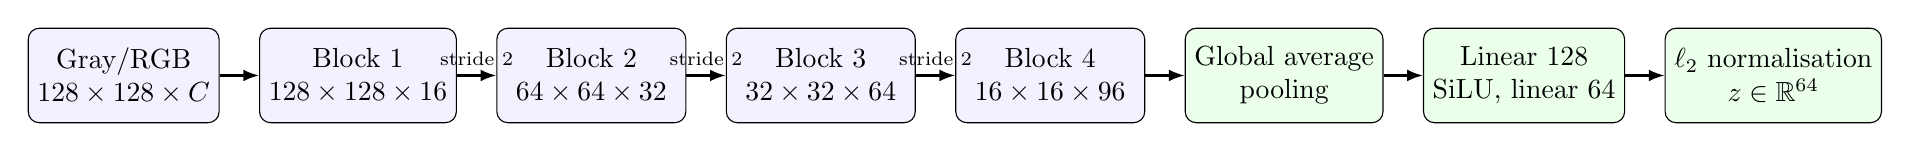
\begin{tikzpicture}[
  node distance=5mm,
  layer/.style={draw, rounded corners, align=center, minimum height=12mm,
    minimum width=24mm, fill=blue!5},
  head/.style={draw, rounded corners, align=center, minimum height=12mm,
    minimum width=21mm, fill=green!8},
  arrow/.style={-{Latex[length=2mm]}, thick}
]
\node[layer] (input) {Gray/RGB\\$128\times128\times C$};
\node[layer, right=of input] (b1) {Block 1\\$128\times128\times16$};
\node[layer, right=of b1] (b2) {Block 2\\$64\times64\times32$};
\node[layer, right=of b2] (b3) {Block 3\\$32\times32\times64$};
\node[layer, right=of b3] (b4) {Block 4\\$16\times16\times96$};
\node[head, right=of b4] (gap) {Global average\\pooling};
\node[head, right=of gap] (proj) {Linear 128\\SiLU, linear 64};
\node[head, right=of proj] (norm) {$\ell_2$ normalisation\\$z\in\mathbb{R}^{64}$};
\draw[arrow] (input)--(b1);
\draw[arrow] (b1)--node[above, font=\scriptsize]{stride 2}(b2);
\draw[arrow] (b2)--node[above, font=\scriptsize]{stride 2}(b3);
\draw[arrow] (b3)--node[above, font=\scriptsize]{stride 2}(b4);
\draw[arrow] (b4)--(gap);
\draw[arrow] (gap)--(proj);
\draw[arrow] (proj)--(norm);
\end{tikzpicture}%
}
\caption{Descriptor encoder used in both principal evaluations, with $C=1$
for BOSSBase and $C=3$ for Caltech-101. Each
convolutional block contains two $3\times3$ convolution--batch
normalisation--SiLU stages. Channel transformations precede model resizing.}
\label{fig:encoder}
\end{figure*}

\subsection{Balanced quantile codebook}

Let $Z\in\mathbb{R}^{N\times64}$ contain clean descriptors and let $v_1$ be
the first right singular vector of the centred matrix. Each descriptor is
projected as
\begin{equation}
s_i=(z_i-\bar z)^\top v_1.
\end{equation}
For a candidate alphabet of size $K$, boundaries are placed at the empirical
quantiles $j/K$, $j=1,\ldots,K-1$. The resulting label is
\begin{equation}
q_K(z_i)=\sum_{j=1}^{K-1}\mathbf{1}[s_i>b_j].
\label{eq:quantile}
\end{equation}
Quantile partitioning balances clean occupancy before channel qualification
and avoids empty clusters caused solely by an unconstrained fit. The complete
clean-image assignment is defined by Eq.~\eqref{eq:quantile}.
The first singular direction is used because it is deterministic and captures
the largest descriptor variance with one scalar. In the reduced sensitivity
subset it explained 72.90\% of the variance; the first two directions jointly
explained 96.83\%. Alternative directions occasionally retained more stable
covers, so $v_1$ is treated as a reproducible design choice rather than a
stability optimum.

\subsection{Attack-qualified cover index}

A cover is retained only when its label is unchanged under every calibration
condition:
\begin{equation}
\mathcal{S}_K=
\left\{i:q_K(f_\theta(T(x_i)))=q_K(f_\theta(x_i)),
\ \forall T\in\mathcal{T}_{\mathrm{cal}}\right\}.
\label{eq:stable}
\end{equation}
The calibration set contains 12 transformations: JPEG qualities 80 and 50;
Gaussian noise with standard deviations 5 and 12; Gaussian blur radii 0.8 and
1.5; resize factors 0.75 and 0.50; crop fractions 0.05 and 0.10; and rotations
of $3^\circ$ and $7^\circ$.

Stability filtering can introduce visible selection bias. Seven image
statistics are therefore used to estimate the probability that a cover is
stable: mean, standard deviation, horizontal and vertical gradient magnitude,
entropy, and the 0.1 and 0.9 quantiles. Within each symbol bucket, stable
covers are ordered by clipped inverse-propensity weighted random priorities.
This ordering does not change labels or pixels; it reduces deterministic
preference for visually distinctive stable covers.

\subsection{Protected message representation}

For plaintext $m$ and sequence number $n$, AES-GCM
\cite{nist2007gcm} produces
\begin{equation}
c=\operatorname{AEAD.Enc}_{k_p}(m;\mathrm{nonce},
\texttt{NARCIS-PAYLOAD-1}\Vert n).
\end{equation}
The ciphertext envelope is framed with a protocol marker, length, and CRC-32,
then encoded with Reed--Solomon parity \cite{reed1960polynomial}. Session metadata contains the sequence
number, padding, codebook size, and cover count. It is independently sealed
with AES-GCM using sender and receiver identities as associated data. The
receiver accepts only a sequence number greater than the highest previously
accepted value for that sender.

For $K=2^b$, the coded bit stream is divided into $b$-bit symbols. A keyed
permutation combines a Gray ordering, a key-derived cyclic shift, and a
key-derived orientation. Adjacent symbol values consequently remain adjacent
in the unshifted codebook order, while the externally observed symbol-to-label
assignment depends on the key.

More precisely, let
$h=\operatorname{HMAC\mbox{-}SHA256}(k_s,\texttt{cluster-order})$
\cite{nist2008hmac},
$a=\operatorname{int}(h_{0:8})\bmod K$, and
$r=-1$ if the least significant bit of $h_8$ is one, otherwise $r=1$.
For position $p\in\{0,\ldots,K-1\}$, define the binary-reflected Gray symbol
$g(p)=p\oplus(p\!\gg\!1)$ and
\begin{equation}
\pi_k(g(p))=(a+rp)\bmod K.
\label{eq:keyedgray}
\end{equation}
The sender maps each coded symbol through $\pi_k$; the receiver constructs
the exact inverse table. Equation~\eqref{eq:keyedgray} fully specifies the
mapping and separates its role from payload encryption.

\subsection{Feasible operating point}

Let $d_k(c)$ denote the number of occurrences of label $k$ required to
transmit protected envelope $c$, and let $a_k$ be the number of unused
qualified covers in bucket $k$. A candidate codebook is feasible when
\begin{equation}
d_k(c)\leq a_k,\qquad
\forall k,\ \forall c\in\mathcal{C}_{\mathrm{eval}}.
\label{eq:feasibility}
\end{equation}
Candidate sizes are evaluated from the largest to the smallest. The selected
operating point is the largest $K$ satisfying Eq.~\eqref{eq:feasibility}.
This criterion distinguishes nominal symbol capacity $\log_2K$ from the net
payload rate after encryption, framing, and error correction.

\subsection{Computational complexity}

Let $N$ be the index size, $A=|\mathcal{T}_{\mathrm{cal}}|$, $d$ the
descriptor dimension, $K$ the alphabet size, $L$ the number of transmitted
covers, and $F_\theta$ the cost of one encoder inference. Clean embedding
costs $O(NF_\theta)$. Multi-attack qualification is the dominant offline term,
$O(ANF_\theta+ANKd)$ when label assignment is written explicitly. The scalar
quantile implementation reduces label assignment after projection to
$O(AN\log K)$ through binary search over the ordered boundaries.
PCA fitting costs $O(Nd^2)$ for $N\ge d$, and sorting the projected values
costs $O(N\log N)$. Online cover retrieval and keyed mapping are $O(L)$ with
pre-built buckets, while decoding adds the Reed--Solomon block cost. Storage
is $O(Nd+N)$ for descriptors and indexed identifiers. Offline qualification
is therefore intentionally amortised across subsequent transmissions.

Figure~\ref{fig:pipeline} separates offline index construction from online
protected transmission and recovery.

\begin{figure*}[t]
\centering
\resizebox{\textwidth}{!}{%
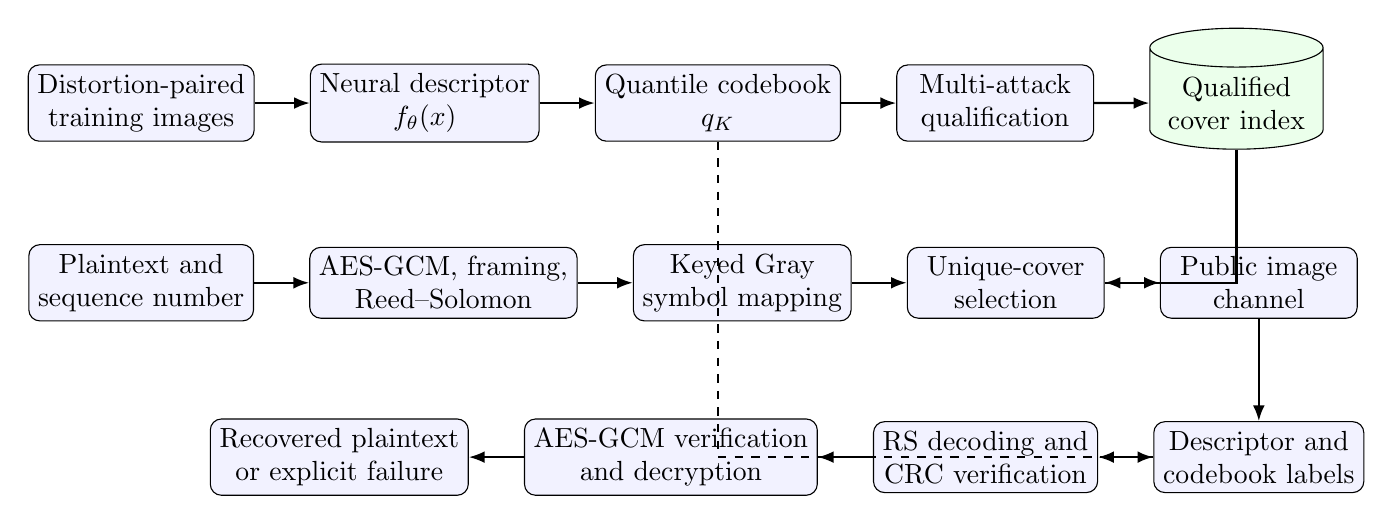
\begin{tikzpicture}[
  node distance=5mm and 7mm,
  box/.style={draw, rounded corners, align=center, minimum height=9mm,
    minimum width=25mm, fill=blue!5},
  store/.style={draw, cylinder, shape border rotate=90, aspect=0.25,
    align=center, minimum height=11mm, minimum width=22mm, fill=green!8},
  arrow/.style={-{Latex[length=2mm]}, thick},
  dashedarrow/.style={-{Latex[length=2mm]}, thick, dashed}
]
\node[box] (train) {Distortion-paired\\training images};
\node[box, right=of train] (encoder) {Neural descriptor\\$f_\theta(x)$};
\node[box, right=of encoder] (quantile) {Quantile codebook\\$q_K$};
\node[box, right=of quantile] (qualify) {Multi-attack\\qualification};
\node[store, right=of qualify] (index) {Qualified\\cover index};

\node[box, below=13mm of train] (payload) {Plaintext and\\sequence number};
\node[box, right=of payload] (aead) {AES-GCM, framing,\\Reed--Solomon};
\node[box, right=of aead] (mapping) {Keyed Gray\\symbol mapping};
\node[box, right=of mapping] (select) {Unique-cover\\selection};
\node[box, right=of select] (channel) {Public image\\channel};

\node[box, below=13mm of channel] (classify) {Descriptor and\\codebook labels};
\node[box, left=of classify] (decode) {RS decoding and\\CRC verification};
\node[box, left=of decode] (decrypt) {AES-GCM verification\\and decryption};
\node[box, left=of decrypt] (output) {Recovered plaintext\\or explicit failure};

\draw[arrow] (train) -- (encoder);
\draw[arrow] (encoder) -- (quantile);
\draw[arrow] (quantile) -- (qualify);
\draw[arrow] (qualify) -- (index);
\draw[arrow] (payload) -- (aead);
\draw[arrow] (aead) -- (mapping);
\draw[arrow] (mapping) -- (select);
\draw[arrow] (index) |- (select);
\draw[arrow] (select) -- (channel);
\draw[arrow] (channel) -- (classify);
\draw[arrow] (classify) -- (decode);
\draw[arrow] (decode) -- (decrypt);
\draw[arrow] (decrypt) -- (output);
\draw[dashedarrow] (quantile) |- (classify);
\end{tikzpicture}%
}
\caption{NARCIS construction and transmission pipeline. Training and index
qualification are performed before communication. The transmitted objects are
unchanged images selected from the qualified index.}
\label{fig:pipeline}
\end{figure*}

Algorithm~\ref{alg:narcis} summarises transmission and recovery.

\begin{algorithm}[t]
\caption{NARCIS protected coverless transmission}
\label{alg:narcis}
\KwIn{Plaintext $m$, sequence $n$, qualified index $\mathcal{I}$, keys}
\KwOut{Recovered plaintext or failure}
Encrypt $m$ with sequence-bound AES-GCM\;
Frame the ciphertext and apply Reed--Solomon coding\;
Select the largest feasible codebook $K$\;
Map coded symbols to labels with the keyed permutation\;
Select one unused qualified cover for each required label\;
Transmit the unchanged cover sequence and sealed metadata\;
Verify metadata and reject replayed sequence numbers\;
Classify received covers and invert the keyed mapping\;
Apply Reed--Solomon decoding and verify CRC\;
Authenticate and decrypt the payload\;
\Return plaintext if every verification succeeds; otherwise failure\;
\end{algorithm}

\section{Experimental Protocol}
\label{sec:experiments}

\subsection{Dataset and partitions}

The principal evaluation uses BOSSBase 1.01 \cite{bas2011boss}, containing
10,000 grayscale photographs at $512\times512$ pixels. The dataset is kept at
native resolution for JPEG, noise, blur, resize, crop, and rotation; the
resulting image is resized to $128\times128$ only at the encoder boundary.
For each seed in $\{11,29,47,71,101\}$, a deterministic permutation provides
2,000 training images and a disjoint 8,000-image cover index.

Cross-dataset validation uses Caltech-101 \cite{fei2004caltech}: 9,144 natural
RGB images from 101 object categories with variable source resolutions. The
channel input is centre-fitted to $256\times256$ in RGB, and the transformed
image is resized to $128\times128$ only at the encoder boundary. Each of the
same five seeds assigns 1,500 images to descriptor training and 7,000
disjoint images to the shared index. Semantic labels are neither used in
training nor in codebook construction.

The encoder is trained separately on each partition for five epochs with
AdamW, batch size 16, learning rate $10^{-3}$, and weight decay $10^{-5}$.
The BOSSBase experiment evaluates ten independently generated eight-byte
plaintexts per seed; Caltech-101 evaluates five. Reed--Solomon coding uses 128
parity bytes. Symbol repetition is set to one; redundancy is instead provided
by byte-level Reed--Solomon parity, which avoids multiplying the required
348--464-cover sequences. For longer payloads, fixed framing and parity
overheads would be amortised, but that regime is not inferred here. The two
principal evaluations comprise 75 protected messages and 1,575
message-condition trials.

CIFAR-100 \cite{krizhevsky2009cifar} is retained only for the controlled
qualification ablation and the matched local-descriptor comparison reported
in Section~\ref{sec:secondary}. That experiment uses three seeds, 2,000
training images, an 8,000-image index, and three messages per seed.

\subsection{Channel conditions and metrics}

The 12 calibration transformations are those in
Eq.~\eqref{eq:stable}. Eight holdout strengths are used only at evaluation:
Gaussian noise with standard deviations 9 and 15; blur radii 1.2 and 1.8;
crop fractions 0.08 and 0.12; and rotations of $5^\circ$ and $9^\circ$.
Together with the clean channel, this gives 21 conditions.

Two metrics are reported:
\begin{enumerate}
\item \emph{symbol accuracy}, the fraction of transmitted covers assigned to
their intended labels after channel processing;
\item \emph{complete-message success}, which is one only when error correction,
CRC verification, authenticated decryption, and plaintext equality all
succeed.
\end{enumerate}

Confidence intervals are two-sided 95\% Student-$t$ intervals over the five
seed-level values. They quantify variation across deterministic partitions;
they do not imply coverage over datasets or untested channels.

\subsection{Baselines and ablations}

The local baselines use a normalised $16\times16$ low-frequency DCT descriptor
and a normalised 64-bin grayscale histogram. They are subjected to the same
quantile partition, calibration attacks, candidate codebook sizes, and
protected-message feasibility rule as \method. This is a controlled descriptor
comparison, not a reproduction of a published complete protocol.

The main ablation removes attack-based cover qualification while retaining
the same neural descriptor, codebook size, protected messages, and decoder.
It is run on the smaller CIFAR-100 protocol to isolate the mechanism at lower
computational cost. A second check confirms the configured repetition factor
of one.

\subsection{Selection detectability}

A deliberately interpretable detector uses seven global image statistics:
mean, standard deviation, two gradient magnitudes, entropy, and two intensity
quantiles. Logistic regression distinguishes selected covers from an equal
number of non-selected index images using a stratified 65/35 train/test split.
A second detector extracts 52 high-pass residual co-occurrence summaries
inspired by rich-model steganalysis \cite{fridrich2012rich} and applies an
ExtraTrees ensemble. A third detector is a lightweight selection CNN with
three convolutional stages (16, 32, and 64 channels), batch normalisation,
spatial averaging, and a binary output. It is trained for eight epochs on
$64\times64$ views using the same split. The area under the ROC curve (AUC)
measures detectability. These tests probe qualification-induced selection
bias at increasing model flexibility. The CNN is not presented as a
reproduction of XuNet or SRNet \cite{xu2016steganalysis,boroumand2018srnet},
whose original task is detecting pixel embedding rather than unchanged-image
selection.

\subsection{Sensitivity and computational measurements}
\label{sec:sensitivity}

A targeted reduced experiment uses seed 11, 500 training images, a
1,500-image index, three epochs, and $96\times96$ model inputs. It compares
descriptor dimensions 32, 64, and 128; loss weights $(25,25,1)$, $(1,1,1)$,
and $(25,10,1)$; and projections on the first three principal directions and
a fixed random direction. This experiment diagnoses design choices and is not
used to replace the five-seed operating point.

Wall-clock measurements include native-image descriptor extraction,
calibration, and complete transmission and recovery. Parameter counts are
reported directly from the implemented models.

\section{Results}
\label{sec:results}

\subsection{Codebook feasibility}

Table~\ref{tab:config} reports the selected BOSSBase configurations. Four
partitions supported 16 symbols, corresponding to 4 bits per cover. Seed 47
supported eight symbols, or 3 bits per cover. Between 30.38\% and 48.73\% of
the index remained stable under all 12 calibration attacks.

\begin{table}[t]
\centering
\caption{Selected BOSSBase operating points on 8,000-image indices.}
\label{tab:config}
\begin{tabular}{rrrrr}
\toprule
Seed & $K$ & Bits/cover & Stable covers & Min. bucket\\
\midrule
11  & 16 & 4 & 2,823 (35.29\%) & 92\\
29  & 16 & 4 & 2,430 (30.38\%) & 61\\
47  & 8  & 3 & 3,898 (48.73\%) & 177\\
71  & 16 & 4 & 2,687 (33.59\%) & 80\\
101 & 16 & 4 & 2,846 (35.58\%) & 99\\
\bottomrule
\end{tabular}
\end{table}

Each protected eight-byte plaintext required 348 covers at 4 bits per cover
and 464 covers at 3 bits per cover. The measured net plaintext rates were
therefore 0.184 and 0.138 bits per transmitted cover. These values include
encryption, framing, and error correction and must not be confused with the
nominal alphabet.

\subsection{End-to-end robustness}

All 1,050 BOSSBase trials succeeded: five seeds, ten messages, and 21
conditions. Mean symbol accuracy was 98.74\%. Figure~\ref{fig:attacks} shows
per-condition means. The two most difficult conditions were holdout crop 0.12
(84.37\%) and holdout rotation $9^\circ$ (91.75\%). The worst individual
symbol accuracy was 81.61\%. Reed--Solomon corrected at most 61 byte
positions, and authenticated decryption recovered every plaintext.

\begin{figure}[t]
\centering
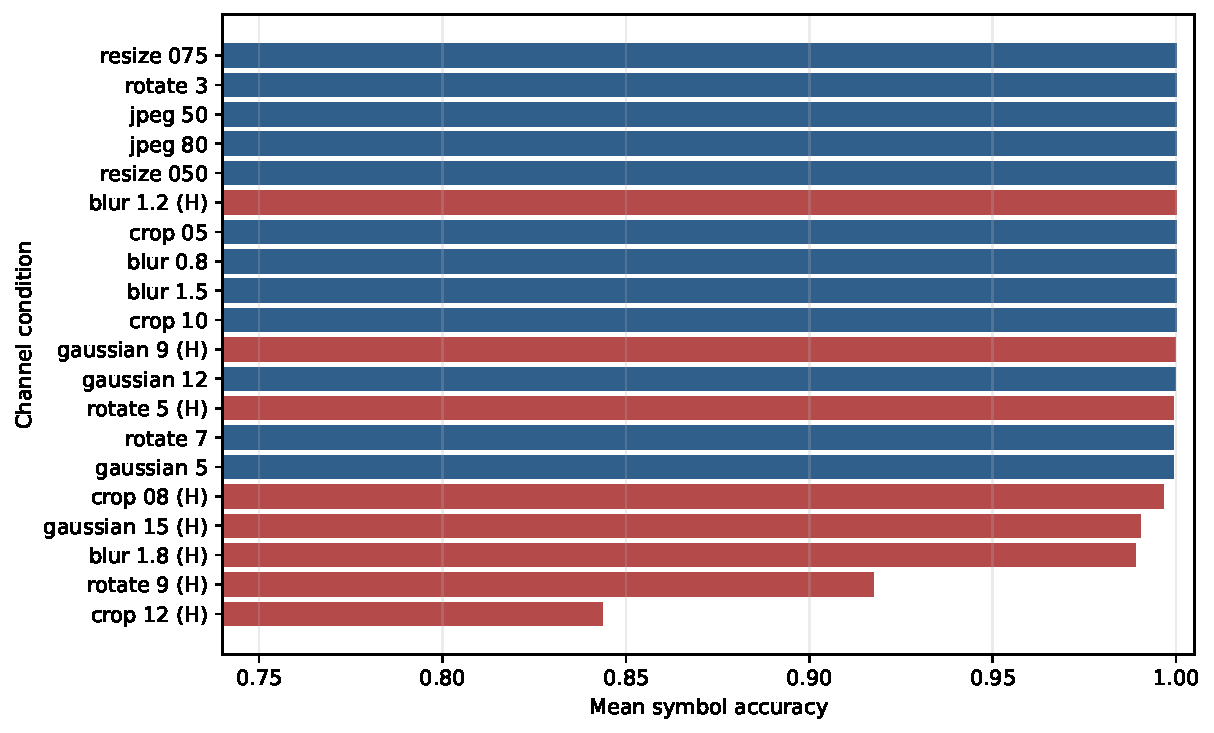
\includegraphics[width=\linewidth]{figures/bossbase_attack_accuracy.pdf}
\caption{Mean BOSSBase symbol accuracy over five seeds and ten messages per
seed. Holdout strengths were excluded from codebook qualification.
Complete-message success was 100\% for every condition.}
\label{fig:attacks}
\end{figure}

The clean channel, both JPEG settings, both resize settings, calibrated crops,
both blur calibration settings, and rotations up to $3^\circ$ produced 100\%
mean symbol accuracy. Message success is not inferred from these averages; it
is verified after Reed--Solomon decoding, CRC checking, and authenticated
decryption.

\subsection{Cross-dataset validation}

All five Caltech-101 partitions selected $K=16$, corresponding to 4 bits per
cover. Table~\ref{tab:caltech} reports the retained-cover statistics. Stable
fractions ranged from 22.00\% to 34.74\%, and every minimum bucket supported
the five protected messages evaluated for its partition.

\begin{table}[t]
\centering
\caption{Selected Caltech-101 operating points on 7,000-image RGB indices.}
\label{tab:caltech}
\begin{tabular}{rrrr}
\toprule
Seed & Bits/cover & Stable covers & Min. bucket\\
\midrule
11  & 4 & 1,678 (23.97\%) & 38\\
29  & 4 & 1,540 (22.00\%) & 31\\
47  & 4 & 2,432 (34.74\%) & 76\\
71  & 4 & 2,289 (32.70\%) & 45\\
101 & 4 & 1,895 (27.07\%) & 35\\
\bottomrule
\end{tabular}
\end{table}

All 525 Caltech-101 message-condition trials recovered the authenticated
plaintext. Mean symbol accuracy was 98.59\%, the worst individual accuracy
was 79.89\% under the unseen 12\% crop, and Reed--Solomon corrected at most
63 byte positions. Figure~\ref{fig:crossrobustness} compares the two datasets
condition by condition. The same holdout crop and rotation remain the hardest
conditions, while dataset-specific differences appear for strong blur.

\begin{figure*}[t]
\centering
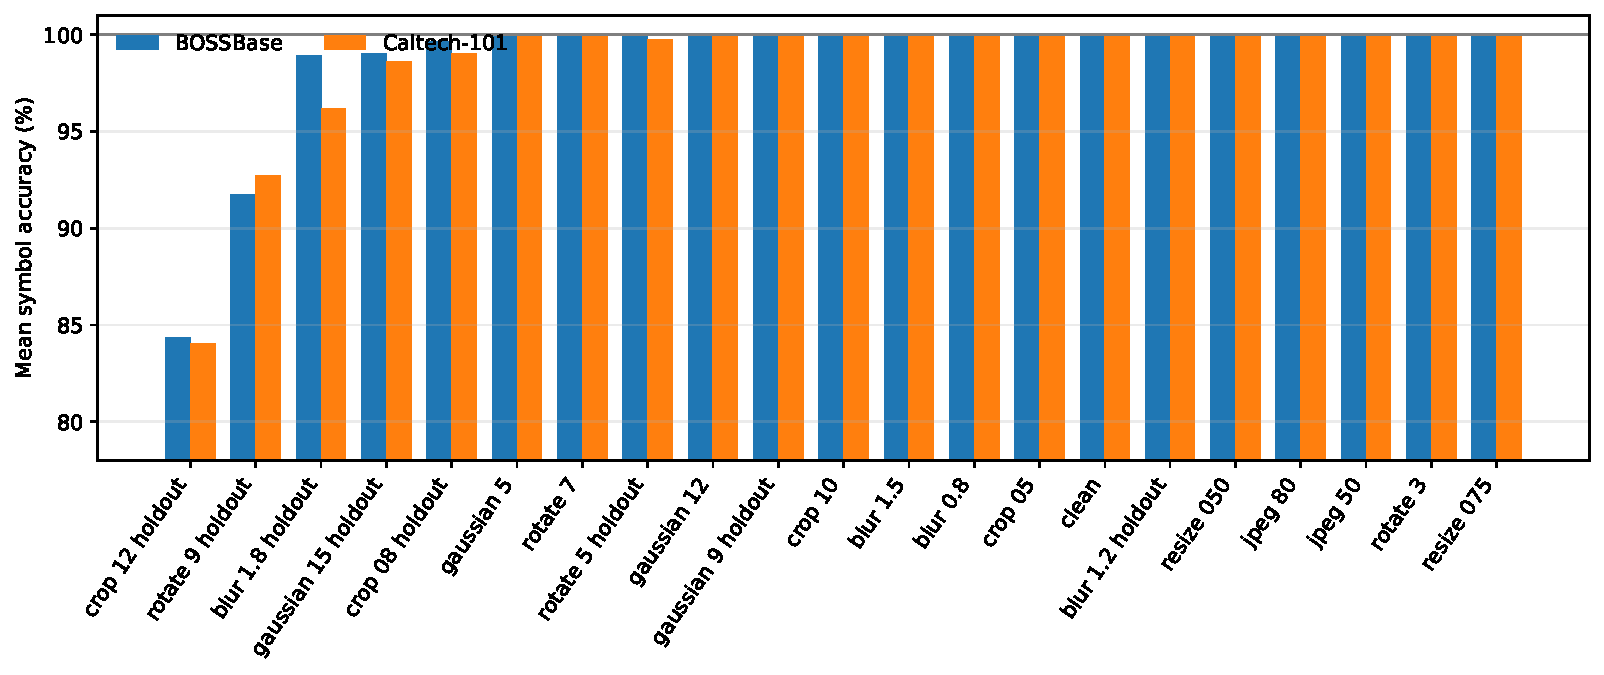
\includegraphics[width=\textwidth]{figures/cross_dataset_robustness.pdf}
\caption{Mean symbol accuracy across the five BOSSBase and five Caltech-101
partitions. Calibration and holdout conditions use the same declared
strengths; all 1,575 complete-message trials succeeded.}
\label{fig:crossrobustness}
\end{figure*}

\subsection{Training convergence}

Figure~\ref{fig:convergence} reports the complete five-epoch histories. Loss
decreased substantially beyond epoch two for every seed. The final values
ranged from 0.066 to 0.157. Individual curves are not monotonic because each
epoch samples new distortion pairs. The experiment supports the use of five
epochs over the earlier two-epoch setting, without asserting asymptotic
convergence.

\begin{figure}[t]
\centering
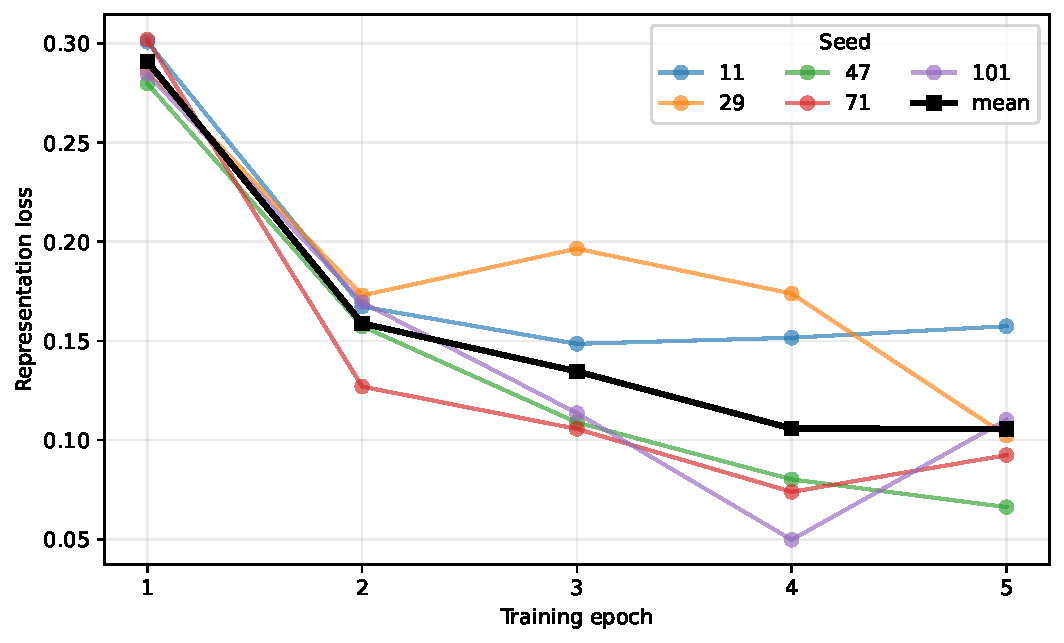
\includegraphics[width=\linewidth]{figures/bossbase_convergence.pdf}
\caption{BOSSBase training loss for the five deterministic partitions.}
\label{fig:convergence}
\end{figure}

\subsection{Selection detectability}

On BOSSBase, the global, residual-ensemble, and CNN detectors produced mean
AUCs of 0.518, 0.514, and 0.515, with 95\% intervals [0.489, 0.547],
[0.486, 0.543], and [0.463, 0.566]. On Caltech-101, the corresponding means
were 0.531, 0.533, and 0.530, with intervals [0.504, 0.557],
[0.504, 0.562], and [0.481, 0.579]. Figure~\ref{fig:detectability} summarises
these results.

The BOSSBase intervals and both CNN intervals include 0.5. The two classical
Caltech-101 detectors show a small but measurable dataset-specific selection
shift, while the more flexible CNN result is less precise and does not exclude
chance. These outcomes motivate reporting selection detectability by dataset
and detector rather than inferring a general undetectability property.

\begin{figure}[t]
\centering
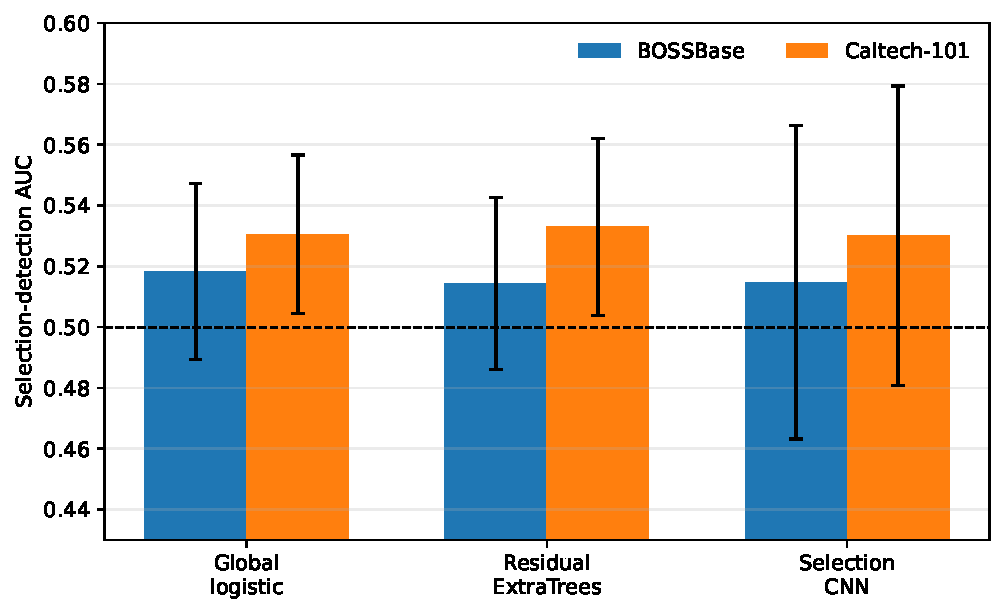
\includegraphics[width=\linewidth]{figures/cross_dataset_detectability.pdf}
\caption{Mean selection-detection AUC and 95\% Student-$t$ intervals over five
partitions per dataset. The dashed line denotes chance performance.}
\label{fig:detectability}
\end{figure}

\subsection{Sensitivity and complexity}

Table~\ref{tab:sensitivity} summarises the reduced sensitivity experiment.
Equal loss weights retained fewer stable covers and produced the smallest
minimum bucket. Dimension 128 improved retained stability in this subset, but
a confirmatory two-seed full-protocol run recovered 419/420 trials, compared
with 420/420 for the corresponding 64-dimensional runs. The 64-dimensional
configuration is therefore retained because the larger representation did not
improve tested capacity or reliability. The one-trial difference is not
interpreted as statistically significant; it only shows that the larger
descriptor provided no observed reliability gain in this limited confirmatory
run.

\begin{table}[t]
\centering
\caption{Targeted sensitivity study on the reduced BOSSBase subset.}
\label{tab:sensitivity}
\begin{tabular}{lrr}
\toprule
Configuration & Stable fraction & Min. bucket\\
\midrule
64D, 25/25/1 & 0.335 & 9\\
32D, 25/25/1 & 0.375 & 19\\
128D, 25/25/1 & 0.412 & 20\\
64D, 1/1/1 & 0.284 & 5\\
64D, 25/10/1 & 0.357 & 19\\
\bottomrule
\end{tabular}
\end{table}

PC1 explained 72.90\% of descriptor variance and retained 33.47\% of covers.
PC2 retained 34.93\%, PC3 31.40\%, and a fixed random direction 41.27\%.
This result rules out a claim that PC1 is stability-optimal. It instead
motivates attack-aware direction selection as a subsequent extension.

Native-image descriptor extraction averaged 87.83 seconds for 8,000 covers,
or 99.85 images/s. Calibration averaged 1,246.10 seconds per partition.
Complete evaluation averaged 754.63 seconds for 210 message-condition trials,
equivalent to 3.59 seconds per trial. Dimensions 32, 64, and 128 contain
218,928, 231,312, and 268,368 parameters, respectively; similar inference
times confirm that the convolutional backbone dominates cost.

\subsection{Secondary ablation and descriptor comparison}
\label{sec:secondary}

The controlled CIFAR-100 experiment recovered 189/189 protected
message-condition trials at $K=16$, with mean symbol accuracy 98.47\%.
Removing attack qualification reduced complete-message success from 100\% to
43.65\% over the matched ablation trials. This identifies qualification as a
necessary robustness component rather than treating invariant training alone
as sufficient.

Under the same quantile partition, attack set, candidate sizes, and
protected-message demand, neither the $16\times16$ DCT descriptor nor the
64-bin histogram formed a feasible codebook in any of three partitions. This
is a controlled descriptor comparison, not a claim against all handcrafted
coverless systems.

\subsection{Position relative to published methods}

Table~\ref{tab:position} separates directly measured properties from published
context. Abdulsattar and WYSAWIS provide high nominal intra-image or
category-based representations \cite{abdulsattar2021,wysawis2025}, whereas
\method evaluates a protected multi-cover sequence. Guo and Ping
\cite{guo2026capacity} report higher nominal capacities and high average
robustness on larger datasets. Their reported capacity is therefore stronger
than the 3--4 bit operating points measured here.

\begin{table*}[t]
\centering
\caption{Positioning of NARCIS. Values from different publications are not
treated as a common-protocol ranking.}
\label{tab:position}
\begin{tabularx}{\textwidth}{p{2.7cm}YYYY}
\toprule
Property & Abdulsattar \cite{abdulsattar2021} & WYSAWIS \cite{wysawis2025} &
Guo--Ping \cite{guo2026capacity} & NARCIS\\
\midrule
Representation & Eigenvalue comparisons in overlapping blocks &
15-bit block hashes grouped into 16 categories &
PZM features with stability-aware quantisation and clustering &
Learned invariant descriptors with quantile codebook\\
Primary capacity statement & High nominal single-cover location capacity &
High nominal block/category capacity &
10, 14, and 15 bits on Holidays, VOC, and ImageNet &
3--4 bits on BOSSBase; 4 bits on Caltech-101\\
Explicit multi-attack cover qualification & Not evaluated here &
Not evaluated here & Yes & Yes\\
Message-level error correction & Not part of the compared mechanism &
Not part of the compared mechanism & Not stated in the reported context &
Reed--Solomon, measured after complete decoding\\
Authenticated payload and metadata & Not part of the compared mechanism &
Not part of the compared mechanism & Not stated in the reported context &
AES-GCM with sequence-bound data and replay guard\\
Holdout attack strengths & Not evaluated here & Not evaluated here &
Not established from the cited summary & Eight holdout strengths\\
Measured complete protected-message recovery & Not evaluated here &
Not evaluated here & Not directly comparable & 1,575/1,575 trials\\
\bottomrule
\end{tabularx}
\end{table*}

\method's advantage is therefore not global capacity. Its supported
positioning is protocol completeness: unchanged-cover signalling, explicit
finite-index feasibility, attack-qualified selection, authenticated
communication, replay control, and complete-message recovery under calibrated
and holdout distortions.

\FloatBarrier
\section{Discussion}
\label{sec:discussion}

\subsection{What the experiments establish}

The experiments support four conclusions. First, stable descriptor averages
are insufficient for communication: the multiplicity of every required
symbol must be checked. Second, cover qualification is the dominant robustness
component in the tested pipeline. Third, forward-error correction allows
message recovery at symbol accuracies substantially below 100\%. Fourth,
cryptographic verification changes the evaluation criterion: a trial is
successful only when the exact plaintext is authenticated and recovered.

The five-seed results also quantify finite-index and cross-corpus variability.
The same rules yield a feasible 16-symbol alphabet on four BOSSBase
partitions and an eight-symbol alphabet on one, while all five Caltech-101
partitions support 16 symbols. Reporting the lower BOSSBase operating point
avoids selecting only favourable partitions.

\subsection{Security interpretation}

AES-GCM, associated data, and monotonic sequence checking provide conventional
confidentiality, authenticity, binding, and replay rejection under correct key
and nonce management. These properties do not conceal communication volume or
image semantics. Distributional detectability is therefore evaluated
separately from cryptographic payload security. The AUC experiment addresses
a different question: whether
the current selection policy creates detectable shifts in seven global
statistics, residual summaries, or a learned CNN representation. The small
classical-detector shift on Caltech-101 and the wider CNN intervals show why
these measurements must remain tied to a dataset, selection policy, and
detector. They do not support a general undetectability claim.

\subsection{Limitations}

The evaluation has four main limitations.

\begin{enumerate}
\item Caltech-101 adds variable-resolution RGB content, but its channel input
is centre-fitted to $256\times256$ for batching. Evaluation on larger
native-resolution colour corpora would test a broader operating regime.
\item The local baselines isolate descriptor feasibility; they are not faithful
reimplementations of complete published systems.
\item The learned selection detector is a lightweight CNN designed for the
selected-versus-non-selected task, not an SRNet reproduction. Traffic-level
sequence analysis is also outside this study.
\item PC1 is reproducible and variance-maximising, but the sensitivity study
shows that attack-aware projection selection may retain more stable covers.
\end{enumerate}

The measured net plaintext rates, 0.184 and 0.138 bits per transmitted cover,
are lower than the nominal symbol capacities because the experiments use
short payloads and 128 parity bytes. This overhead is reported explicitly.
Longer-block efficiency was not measured and is not inferred.

\section{Conclusion}
\label{sec:conclusion}

NARCIS integrates learned image descriptors, balanced codebooks, attack-based
cover qualification, keyed assignment, authenticated encryption, replay
control, and Reed--Solomon correction into one selection-based coverless
protocol. It recovered 1,050 of 1,050 protected message-condition trials on
BOSSBase and 525 of 525 on RGB Caltech-101, including eight holdout attack
strengths. BOSSBase supported 3--4 bits per cover; every Caltech-101 partition
supported 4 bits per cover. Mean symbol accuracies were 98.74\% and 98.59\%.
Removing qualification in the controlled ablation reduced complete-message
success to 43.65\%.

These results support a precise position: NARCIS provides measured robust
operating points and complete protected-message recovery with unchanged
natural covers. Operationally, the results show that finite-index feasibility
and byte-level correction can convert imperfect label stability into exact,
authenticated recovery without modifying transmitted images. The evidence
does not support a global capacity or universal steganalysis claim.

Three extensions follow directly from the observed limits. First,
attack-aware projection selection should be trained on calibration data while
being locked before holdout evaluation. Second, executable recent-protocol
baselines should be evaluated under the same payload protection, attacks, and
finite-index demand. Third, larger native-resolution colour corpora and
traffic-level sequence detectors should extend the present image-level
analysis. These directions target capacity, comparative attribution, and
detectability separately while preserving the feasible-operating-point
criterion as the common evaluation unit.

\section*{Acknowledgements}
This work was supported by the authors' institutions. No external financial
support was received.

\printcredits

\section*{Declarations}
\noindent\textbf{Ethics approval.}
This study does not involve human participants, animals, personal data, or
clinical interventions. It uses publicly available image datasets and offline
computational experiments.

\medskip
\noindent\textbf{Competing interests.}
The authors declare that they have no known competing financial interests or
personal relationships that could have appeared to influence the work
reported in this paper. WYSAWIS, cited in the related work, shares authors
with this study and is identified explicitly. It is used as qualitative
published context, not as an experimental baseline or as evidence for the
numerical claims reported here.

\medskip
\noindent\textbf{Funding.}
This research received no external funding.

\medskip
\noindent\textbf{Data availability.}
BOSSBase 1.01 is publicly available from its original distributor at
\url{https://agents.fel.cvut.cz/boss/}; Caltech-101 is available from
CaltechDATA at \url{https://data.caltech.edu/records/mzrjq-6wc02}; and
CIFAR-100 is available at
\url{https://www.cs.toronto.edu/~kriz/cifar.html}. The datasets are not
redistributed in the project repository.
Deterministic partition seeds and consolidated CSV/JSON results accompany the
reproducibility package.

\medskip
\noindent\textbf{Code availability.}
The NARCIS implementation, attack definitions, evaluation scripts, tests,
consolidated result tables, plotting code, manuscript sources, and exact
random seeds are publicly available at
\url{https://github.com/EkodeckStephane/NARCIS}. Trained checkpoints are not
redistributed; the repository provides the commands required to retrain the
models.

\FloatBarrier
\bibliographystyle{cas-model1-num-names}
\bibliography{cas-refs}

\end{document}
